\section{Systemfunktionen}
\label{system_features}

Wir haben die Systemfunktionen nach Usergruppen aufgeteilt.

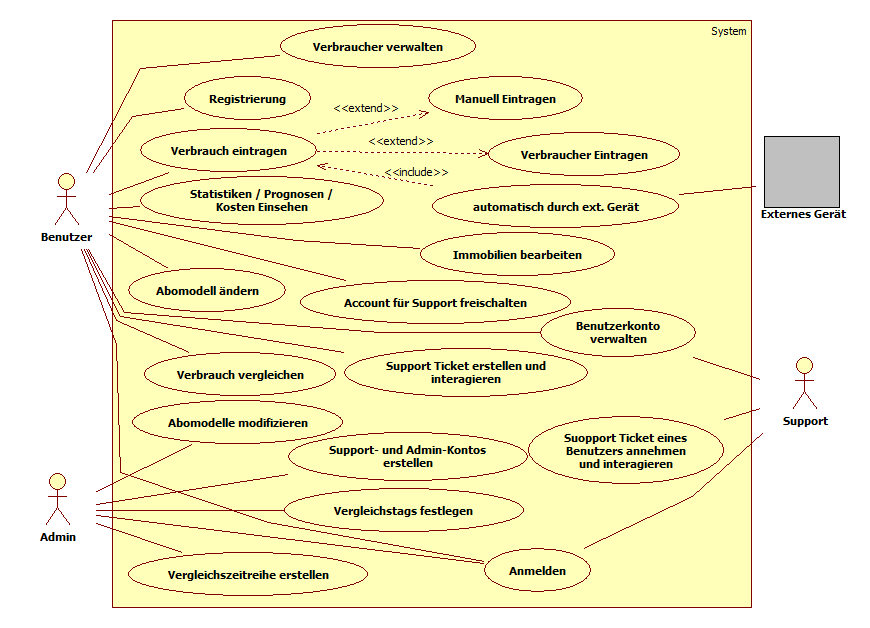
\includegraphics[scale=0.4]{use_case.png}

\subsection{Systemfunktionen für alle Usergruppen}
\subsubsection{Anmeldung}
\paragraph{Beschreibung und Priorität}

Bevor ein dem System bereits bekannter Nutzer Die Funktionen seiner Usergruppe ausführen kann, muss er sich zunächst authentifizieren. Die Funktion hat eine sehr hohe Priorität, da sonst Nutzer und Nutzergruppen nicht voneinander unterschieden werden können.

\paragraph{Sequenzen von Benutzeraktionen und Systemantworten}

Der Nutzer gibt in einer Anmeldemaske seinen Benutzername oder seine Email-Adresse und sein Passwort ein und bestätigt dies. Ist ANM4 erfüllt so ist der Nutzer nun eingeloggt und wird zum Home-Bildschirm weitergeleitet. War dies nicht der Fall, so wird eine Fehlermeldung mit den möglichen Ursachen angezeigt.

\paragraph{Funktionale Anforderungen}
\begin{itemize}
	\item \textbf{ANM1} Darstellen der Anmelde-Maske.
	\item \textbf{ANM2} Validieren den Eingabe also Überprüfung von ANM4 durch ggf. Abgleich mit der Datenbank.
	\item \textbf{ANM3} Auf nicht erfüllte Anforderungen (ANM4) in der Anmeldemaske aufmerksam machen, falls diese nicht erfüllt sind.
	\item \textbf{ANM4} Der Benutzername oder die Email-Adresse muss im System vorhanden sein und das Passwort bzw. dessen Hash müssen übereinstimmen.
\end{itemize}

\subsection{Benutzer}
\subsubsection{Accounterstellung}\label{acc}
\paragraph{Beschreibung und Priorität}
Diese Funktion ermöglicht es, einer Person, die an dem Produkt interessiert ist, ein Account anzulegen und somit anfangen kann das Produkt zu nutzen. Die Priorität dieser Funktion kann nicht überschätzt werden, da ohne sie, keine der Folgenden umsetzbar wäre.
\paragraph{Sequenzen von Benutzeraktionen und Systemantworten} Der/die Interessierte gibt in der Anmelde-Maske ihren frei gewählten Benutzername, ihre E-Mail-Adresse und schließlich ein Passwort ein. Nach einem Knopfdruck, wird, wenn die Eingaben die funktionalen Anforderungen REG4, REG5, REG6 erfüllen, der Benutzer nun auf die Startseite weitergeleitet. Wenn nicht, wird der Benutzer über die nicht erfüllten Anforderungen in der Anmelde-Maske informiert und kann daraufhin seine/ihre Eingaben anpassen.
\paragraph{Funktionale Anforderungen}
\begin{itemize}
	\item \textbf{REG1} Darstellen der Anmelde-Maske
	\item \textbf{REG2} Validieren den Eingabe also Überprüfung von REG4, REG5, REG6  durch ggf. Abgleich mit der Datenbank
	\item \textbf{REG3} Auf nicht erfüllte Anforderungen (REG4, REG5, REG6) in der Anmeldemaske aufmerksam machen, falls diese nicht erfüllt sind.
	\item \textbf{REG4} Kein 2 Benutzer dürfen den selben Benutzername haben.
	\item \textbf{REG5} Das Passwort muss dem folgenden Standard genügen:
	      \begin{itemize}
		      \item Mindestlänge: 8 Zeichen
		      \item Enthält min. einen deutschen Großbuchstaben (A-Z, Ä, Ö, Ü)
		      \item Enthält min. einen deutschen Kleinbuchstaben (a-z, ä, ö, ü, ß)
		      \item Enthält min. eine arabische Ziffer (0-9)
		      \item Enthält min. ein Zeichen, dass nicht in die bisherigen Kategorien passt (!, \$, \#, \%, ...)
	      \end{itemize}
	\item \textbf{REG6} Die eingegebene E-Mail-Adresse muss im richtigen Format sein.
	\item \textbf{REG7} Abspeichern der neuen Accountdaten.

\end{itemize}

\subsubsection{Verbräuche eintragen}
\label{sysf:verb_eintragen}
\paragraph{Beschreibung und Priorität}
Es ermöglicht dem Benutzer seine Daten in die Datenbank einzutragen, welche später für weitere Features von Nöten sind. Neben dem manuellen Eintragen gibt es auch die Möglichkeit der automatischen Erfassung der Daten mittels einem Gerät, das der Benutzer zuhause installieren muss, sobald dies passiert ist übermittelt das Gerät jeden Tag die aktuellen Daten… oder so.

\paragraph{Sequenzen von Benutzeraktionen und Systemantworten}
Der Benutzer trägt in einer WebMaske seine einzelnen Verbräuche ein und kann mit einem Klick auf den Button “hochladen” seine Daten der Datenbank hinzufügen, bevor dies geschieht, wird aber überprüft, ob die Daten neu und sinnig sind.
\paragraph{Funktionale Anforderungen}
Noch zu diskutieren.

\subsubsection{Statistiken einsehen}
\paragraph{Beschreibung und Priorität}
Die Funktion ermöglicht es dem Benutzer seine eingetragenen Verbräuche (siehe \ref{sysf:verb_eintragen}) zu visualisieren. Da dieses Funktion den meisten Nutzen für die Benutzer bringt, hat auch diese Funktion eine hohe Priorität, sie ist aber nicht essentiell für das Funktionieren des Systems.

\paragraph{Sequenzen von Benutzeraktionen und Systemantworten}

Der Nutzer geht auf den Menüpunkt Statistiken und wählt den gewünschten Verbrauchszeitraum und die Verbrauchsart aus. Außerdem kann er sich für eine Art der Visualisierung (z.B. Säulendiagramm, Liniendiagramm, oder Tabelle) entscheiden. Die gewünschten Daten werden daraufhin dargestellt.

\paragraph{Funktionale Anforderungen}
Noch zu diskutieren.

\subsubsection{Prognosen einsehen}
\paragraph{Beschreibung und Priorität}
Die Funktion Prognosen einsehen dient dem Nutzer dazu Prognosen für zukünftige Verbräuche einzusehen. Die Prognosen werden auf Basis von vorherigen Verbräuchen und eingetragenen Verbrauchern gebildet. Wenn der Verbauch eines Nutzers im letzten Jahr ungefähr gleich geblieben ist, wird dies auch für das nächste Jahr prognostiziert.
\paragraph{Sequenzen von Benutzeraktionen und Systemantworten}
Wenn der Nutzer sich Prognosen für seine Verbräuche anzeigen lassen möchte, muss er zunächst einen vorhandenen Verbrauchstyp auswählen. Zusätzlich dazu muss der Nutzer einen bestimmten Zeitraum wählen, für die er die Prognose möchte. Falls dieser Zeitraum zu weit in der Zukunft liegt, oder der Verbrauchstyp kaum oder gar keine Verbräuche besitzt, können keine Prognosen ermittelt werden. Wenn Prognosen ermittelt werden können, werden diese dem Nutzer angezeigt. Ob diese Prognosen in Form eines Gesamtverbrauchs (z.B. 1600 kWh für nächstes Jahr), oder in Form einer Verbrauchszeitreihe (Diagramm) angezeigt werden ist noch offen.
\paragraph{Funktionale Anforderungen}
Noch zu diskutieren

\subsubsection{Kosten einsehen}
\paragraph{Beschreibung und Priorität}
Die Funktion Kosten einsehen ermöglicht dem Nutzer die Kosten zu seinen Verbräuchen einzusehen. Bevor dies geschehen kann, muss der Benutzer einen Preis pro angegbener Einheit angeben. Zudem kann er sich bei eigenen Verbrauchstypen auch eigene Kosten eintragen. Beispiel: Der Nutzer hat den Verbrauchstyp Anzahl an Kaffee pro Tag. Dazu kann der Nutzer nun einen Preis eintragen: Ein Kaffee kostet einen Euro.
\paragraph{Sequenzen von Benutzeraktionen und Systemantworten}
Der Nutzer muss einen Verbrauchstyp auswählen und dann zu diesem Typ einen Zeitraum und Kosten pro Einheit wählen. Danach werden ihm die Kosten für den Verbrauch über den Zeitraum angezeigt. Wenn der Nutzer seinen Verbrauch vergleicht, ist neben dem Vergleich des Verbrauchs auch ein Vergleich der Kosten sichtbar.
\paragraph{Funktionale Anforderungen}
Noch zu diskutieren

\subsubsection{Immobilien bearbeiten}
\paragraph{Beschreibung und Priorität}
Der Benutzer kann Immobilien hinzufügen,
bearbeiten und entfernen. %was soll das noch können?
% Ein Benutzer sollte(?) für das Eintragen von Wasser-/Gas-/ Stromverbrauch 
% mindestens eine Immobilie angeben mit Informationen über den Flächeninhalt 
% und Anzahl der Haushaltsmitglieder für eine möglichst genaue Analyse über den Verbrauch des Nutzers verglichen mit dem Durchschnitt. 
Diese Funktion hat keine hohe Priorität(?) da sie nur für den Vergleich mit dem Durchschnitt relevant ist.
\paragraph{Sequenzen von Benutzeraktionen und Systemantworten}
Der Benutzer wählt in seinem Profil aus,
dass er seine Immobilien bearbeiten möchte.
Dabei bekommt er die Option, eine neue Immobilie anzulegen,
oder von vorhandenen Immobilien eine zu bearbeiten.
Wenn er das erste aussucht, kann man eine Bezeichnung,
Flächeninhalt und Haushaltsgröße % noch was?
eintragen. Die Bezeichnung ist zwingend notwendig, %(?)
die anderen Angaben nicht.
Der Nutzer kann sich dazu entscheiden, den Vorgang abzubrechen.
Wenn der Nutzer eine vorhandene Immobilie bearbeiten will,
dann werden ihm ebenfalls angeboten, Bezeichnung, Flächeninhalt und
Haushaltsgröße zu ändern,
zusätzlich hat er die Option, die ganze Immobilie zu löschen.
Wenn der Nutzer etwas bearbeitet hat, bekommt er die Option, seine Änderungen zu speichern.
Wenn er das auswählt, dann ist der Bearbeitungsvorgang abgeschlossen.

Wenn der Nutzer sich für das Löschen entscheidet, wird er final gewarnt,
dass das Löschen einer Immobilie alle damit verbundenen Daten löscht und der Vorgang nicht widerrufbar ist.
%klingt momentan sehr dumm muss geändert werden
Wenn der Nutzer zugestimmt hat, dass ihm das bewusst ist und trotzdem fortfahren will, dann wird die Immobilie und alle Daten die damit verbunden waren aus der Datenbank entfernt.

\paragraph{Funktionale Anforderungen}
Noch zu diskutieren.

% Müssen wir dazu schreiben, was das Character Limit ist? 
%dass Flächen  und Haushaltsgröße nur mit Zahlen angegeben werden können? 
%Was wir mit ungültigen Antworten machen?
\begin{itemize}
	\item Wenn noch keine Immobilie angelegt wurde, gibts auch keine Option, etwas bearbeiten zu können (?)
	\item Die Bezeichnung kann alle möglichen ASCII-Zeichen (?) beinhalten.
	\item Der Flächeninhalt kann nur in positiven Fließkommazahlen/ ganzen Zahlen angegeben werden.
	\item Die Haushaltsgröße kann nur in positiven ganzen Zahlen angegeben werden
	\item ???
\end{itemize}

\subsubsection{Abomodell ändern}
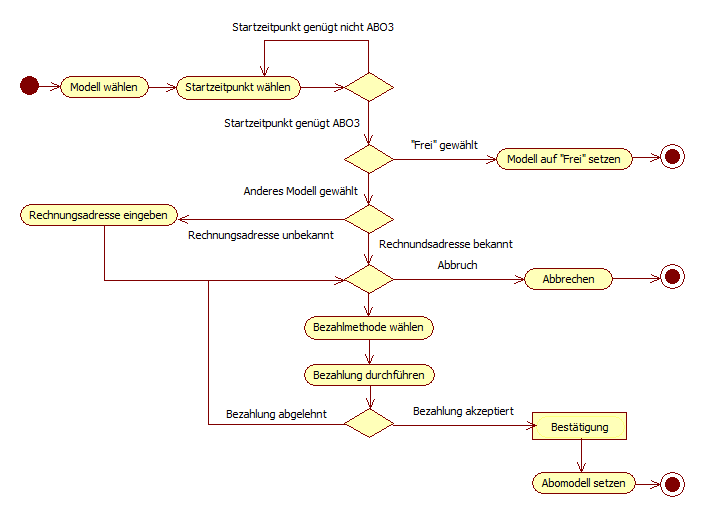
\includegraphics[scale=0.5]{activity_abo.png}


\paragraph{Beschreibung und Priorität}
Der Benutzer kann hiermit zwischen Abomodellen wechseln. Geplant sind die Abomodelle \textit{Frei}, \textit{Standard} und \textit{Professionell} wovon Ersteres kostenlos und standardmäßig ausgewählt sein sollte. Diese Funktion enthält neben dem Auswählen des Modells die Zahlung und Überprüfung vertraglicher Kündigungsfristen. Die Funktion gehört nicht zu den Kernanforderungen jedoch kann ohne Sie kein Umsatz erzielt werden und hat daher trotzdem eine hohe Priorität.
\paragraph{Sequenzen von Benutzeraktionen und Systemantworten}
Nach der Auswahl des gewünschten Abomodells, muss, falls sich der User für ein kostenpflichtiges Modell entscheidet, man einen Startzeitpunkt (nach Richtlinie ABO3) entscheiden. Nach der Eingabe von Rechnungsadresse, die, falls Sie für den Benutzer schon bekannt ist, auch schon vor eingetragen sein sollte, kann der Benutzer eine präferierte Zahlungsmethode anwählen, wodurch er/sie zu einem externen Zahlungsdienstleister weitergeleitet wird. Schließlich kann der Prozess abgeschlossen werden und das neue Abomodell wird zum angegebenen Startzeitpunkt gesetzt. Eine Bezahlbestätigung wird versendet. Der Vorgang kann zu jedem Zeitpunkt abgebrochen werden.

\paragraph{Funktionale Anforderungen}
\begin{itemize}
	\item \textbf{ABO1} Darstellen der Maske zum Auswählen des Abomodells und Eintragen von Startzeitpunkt und Rechnungsdresse.
	\item \textbf{ABO2} Validieren der Eingabe des Startzeitpunkts (nach ABO3) und Reflektieren möglicher Fehler in der Maske
	\item \textbf{ABO3} Der Startzeitpunkt muss folgenden Richtlinien genügen:
	      \begin{itemize}
		      \item Er muss in der Zukunft liegen oder am derzeitigen Tag sein
		      \item Falls die Kündigungszeitraum eines laufendes Abos noch nicht abgelaufen ist, muss der Startzeitpunkt nach Ablauf dieses Zeitraums liegen
	      \end{itemize}
	\item \textbf{ABO4} Grundlegende Format-Überprüfungen der Rechnungsadresse (zB Postleitzahl besteht aus Zahlen etc.) und sollen bei Nichteinhaltung in der Maske kommuniziert werden
	\item \textbf{ABO5} Eine Verbindung zu sämtliche externen Zahlungsanbietern muss aufgebaut werden. Derzeit sind \textit{PayPal}, per Lastschrift, Sofort-Überweisung der \textit{Sofort GmbH}, \textit{Klarna}, mit Kreditkarte ???
	\item \textbf{ABO6} Schaffen einer Möglichkeit in jedem Schritt den Prozess abzubrechen
	\item \textbf{ABO7} Versenden einer Bezahlbestätigung
	\item \textbf{ABO8} Setzen des neuen Abomodells in den Benutzerdaten zum angegebenen Startzeitpunkt
\end{itemize}

\subsubsection{Account für Support freischalten}
\label{sys_feat:freischalten}
\paragraph{Beschreibung und Priorität}
Diese Funktion ermöglicht es dem Benutzer bei Problemen seinen Account für den Support freizuschalten, sodass der Support Änderungen vornehmen kann und gleichzeitig wird so die DSGVO eingehalten, was sehr wichtig für das System ist.
\paragraph{Sequenzen von Benutzeraktionen und Systemantworten}
Der Benutzer hat mit der Nutzung des Systems ein Problem und benötigt Hilfe. Nachdem er das FAQ zur Handhabung des Systems gelesen hat und er dort keine Lösung für sein Problem finden konnte, nutzt er die Supportfunktion, wo er mit einem Mitarbeiter in Kontakt kommt. Zuerst versucht der Support dem Nutzer ohne weitere Daten weiterzuhelfen, sollte dies das Problem immer noch nicht lösen, muss der Nutzer seinen Account für den Support freischalten. Dem Nutzer wird ein Code generiert, den er dem Support durch gibt und den der Support benötigt, um sich berechtigten Zugang zum Nutzeraccount zu verschaffen. Nun kann der  Support dem Nutzer optimal weiterhelfen, indem er Zugriff auf seinen Account hat.
\paragraph{Funktionale Anforderungen}
\begin{itemize}
	\item \textbf{REG1} Laufende Internet- und/oder Telefonverbindung.
	\item \textbf{REG2} Der generierte Code für den Nutzer besteht aus Zahlen und Buchstaben.
	\item \textbf{REG3} Der generierte Code von Nutzer muss unbedingt mit dem benötigten Code des Supports übereinstimmen.

\end{itemize}

\subsubsection{Account verwalten}
\paragraph{Beschreibung und Priorität}
Das Feature erlaubt es dem Nutzer seine Accountdaten einzusehen, zu ändern und gegebenenfalls zu löschen. Das Feature hat eine sehr hohe Priorität.

\paragraph{Sequenzen von Benutzeraktionen und Systemantworten}
Der Nutzer wählt den Menüpunkt \gquote{Account Verwalten} aus. Dort sind alle Optionen AVW1 - AVW6 einsehbar und änderbar.

\paragraph{Funktionale Anforderungen}
\begin{itemize}
	\item \textbf{AVW1} Name
	\item \textbf{AVW2} Adresse
	\item \textbf{AVW3} Zahlungsmethode
	\item \textbf{AVW4} Nutzername
	\item \textbf{AVW5} Email
	\item \textbf{AVW6} Passwort. Hier sollte das aktuelle Passwort jedoch nicht einsehbar sein (da es nicht gespeichert werden soll).
\end{itemize}

\subsubsection{Verbrauch vergleichen}
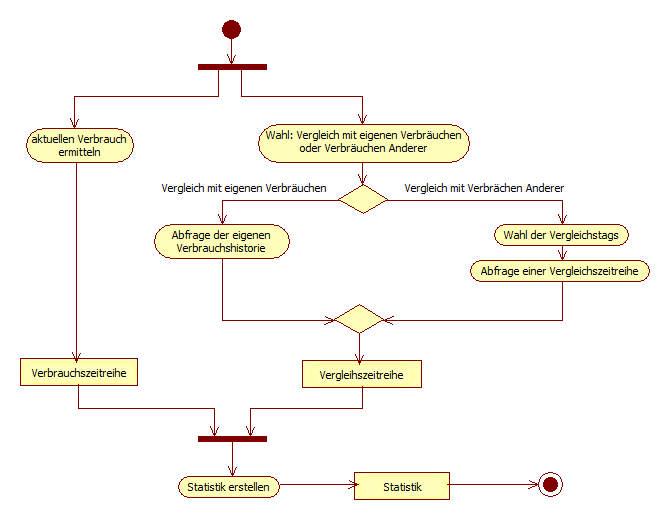
\includegraphics[scale=0.5]{activity_vergleich.png}
% Bei Abfrage einer Vergleichszeitreihe auch darauf eingehen, dass diese auch von extern gekommen sein könnte
\paragraph{Beschreibung und Priorität}
Die Funktion Verbrauch vergleichen ermöglicht dem Nutzer seinen Verbrauch mit seiner eigenen Verbrauchshistorie, oder mit den Verbräuchen anderer zu vergleichen. Falls man sich mit den Verbräuchen von anderen vergleichen möchte, kann man Vergleichstags auswählen (\ref{sec:vergl_tags}). Dann wird eine Vergleichszeitreihe neben der eigenen Verbrauchszeitreihe visualisiert.
\paragraph{Sequenzen von Benutzeraktionen und Systemantworten}
Zunächst muss der Nutzer einen Verbrauchstyp auswählen. Danach wählt der Nutzer aus, ob er sich mit seinen eigenen Verbräuchen, oder mit den Verbräuchen anderer vergleichen möchte. Möchte er sich nur mit sich selber vergleichen, wählt der Nutzer diese Funktion und zwei Zeiträume aus, die er gegeneinander vergleichen möchte. Daraus werden zwei Zeitreihen generiert, die dann in einer Statistik visualisiert werden. Möchte der Nutzer sich mit anderen vergleichen wählt  Vergleichstags (\ref{sec:vergl_tags}). Beispiel: Der Nutzer möchte sich regional Vergleichen, dann kann der Nutzer einen Längenparameter angeben, in welchem Umkreis der Nutzer sich vergleichen möchte. Auch hier muss der Nutzer einen Zeitraum wählen in dem der Nutzer sich vergleichen will. Dann wird eine Vergleichszeitreihe mit der Vergleichsgruppe in dem gegebenen Zeitraum erstellt und visualisiert.
\paragraph{Funktionale Anforderungen}
Noch zu diskutieren

\subsubsection{Support-Ticket erstellen und interagieren!!}
% Hier also auch Support-Ticket Schließen
\paragraph{Beschreibung und Priorität}
Dem Benutzer wird die Möglichkeit gegeben, Support Tickets zu erstellen und somit Kontakt zu einem Supporter aufzunehmen der ihm gegebenenfalls bei einem Problem bezüglich der Software helfen kann. Diese Funktion ist relevant um die Benutzerfreundlichkeit weiter zu erhöhen.
\paragraph{Sequenzen von Benutzeraktionen und Systemantworten}
Der Benutzer wählt den Knopf um den Support zu kontaktieren. Hier hat er die Möglichkeit sein Problem schon konkreter zu schildern. Nach anschließender Bestätigung durch einen weiteren Knopfdruck wird das Ticket erstellt und der Benutzer erhält eine Benachrichtigung, dass sich zeitnah jemand um seine Angelegenheit kümmern wird. Sobald ein Supporter Zeit hat sich dem Problem anzunehmen, kann der Supporter das Ticket annehmen (siehe \ref{ticket_annehmen}) und ein Live Chat zwischen beiden wird eingerichtet. Wenn sich das Problem erledigt hat, hat der Supporter die Möglichkeit den Live Chat zu schließen.
\paragraph{Funktionale Anforderungen}
\begin{itemize}
\item \textbf{TICK1} Bereitstellung eines Interfaces um das Ticket zu erstellen.
\item \textbf{TICK2} Möglichkeit für den Supporter den Live Chat zu schließen.
\end{itemize}


\subsection{Support}
\subsubsection{Support-Ticket eines Benutzers annehmen und interagieren!!}
% Hier kann einfach nach akzeptieren gesagt werden siehe 4.2.11 und auch ein verweis auf 4.3.2 wäre gut.

\subsubsection{Account eines Users verwalten}
\paragraph{Beschreibung und Priorität}
Ein Support-Benutzer muss in der Lage sein etwaige Benutzerdaten auf Anfrage des jeweiligen Benutzers zu ändern. Dafür muss allerdings das Einsehen der Benutzerdaten für den Support freigeschaltet werden (siehe \ref{sys_feat:freischalten}). Diese Funktion ist nicht teil der Kernanforderungen, jedoch muss es unbedingt Teil der ersten Version sein, da die Kundenzufriedenheit davon abhängig ist. Daher ergibt sich eine mittlere Priorität.
\paragraph{Sequenzen von Benutzeraktionen und Systemantworten}
Der Support-Benutzer kann den Benutzer auswählen, dessen Stammdaten bearbeitet werden soll. Dabei werden dem Support-Benutzer nur diejenige Benutzernamen angezeigt, die die Bearbeitung freigeschaltet haben. Danach wird eine Oberfläche angezeigt, die der Oberfläche vom Bearbeiten der eigenen Stammdaten eines Benutzers ähnelt. Hier können nun die Änderungen vorgenommen und gespeichert werden.
\paragraph{Funktionale Anforderungen}
\begin{itemize}
	\item \textbf{SMG1} Zeige alle Benutzer, die die Bearbeitung nach \ref{sys_feat:freischalten} freigeschaltet haben.
	\item \textbf{SMG2} Bearbeiten aller Stammdaten eines Benutzers in der Oberfläche ermöglichen.
	\item \textbf{SMG3} Speichern der veränderten Daten.
\end{itemize}

\subsection{Admin}
\subsubsection{Abomodelle modifizieren}
\paragraph{Beschreibung und Priorität}
Der Admin kann hiermit alle drei verfügbaren Abomodelle (Frei, Standard und Professionell) grundlegend ändern. Alle Abomodelle haben verschiedene Funktionen, welche der Admin anpassen kann. Der Admin hat die Möglichkeit die Kosten der verschieden Modelle anzupassen, Funktionen freischalten und Funktionen einschränken oder sogar ganz entfernen. Falls der Admin die Kosten eines Modells ändert, oder Funktionen hinzufügt oder entfernt, müssen gesetzliche Regelungen für Vertragsänderungen eingehalten werden. Das heißt Nutzer dieses Abomodells müssen benachrichtigt werden und es muss Ihnen eine Möglichkeit gegeben werden, das Abomodell zu kündigen. Das passiert unabhängig davon, ob der Admin die Kosten erhöht oder verringert, oder Funktionen hinzufügt oder entfernt.
\paragraph{Sequenzen von Adminaktionen und Systemantworten}
Falls der Admin Abomodelle modifizieren will, muss der Admin gemäß ABOM3 einen Startzeitpunkt wählen, ab dem die Änderungen gültig werden. Dem Admin soll bekannt gemacht werden, ob der Zeitpunkt zu Nahe gewählt ist. Danach kann der Admin aus folgenden Funktionen wählen:
\begin{itemize}
	\item Vorhanden Funktion bearbeiten oder entfernen (Funktion muss in dem Abomodell momentan verfügbar sein).
	\item Eine neue Funktion hinzufügen
	\item Den Preis des Abomodells ändern
\end{itemize}
Wenn der Admin sich für eine der Funktionen entschieden hat, kann er diese ausführen und bestätigen sofern alles den Anforderungen entspricht. Der gesamte Vorgang kann jederzeit auch abgebrochen werden. Fährt der Admin fort, speichert das System die Änderungen und wendet diese zu dem gegebenen Zeitpunkt an.

\paragraph{Funktionale Anforderungen}
\begin{itemize}
	\item \textbf{ABOM1} Darstellen der Maske zum Auswählen des Abomodells und Eintragen von Startzeitpunkt.
	\item \textbf{ABOM2} Funktion entsprechend dem gewählten Abomodell muss änderbar und löschbar sein
	\item \textbf{ABOM3} Funktion soll hinzufügbar sein.
	\item \textbf{ABOM4} Ein neuer Preis für das Abomodell soll wählbar sein.
	\item \textbf{ABOM5} Der Startzeitpunkt muss in der Zukunft liegen und muss den gesetzlichen Regelungen entsprechen
	\item \textbf{ABOM6} Validieren der Eingabe des Startzeitpunkts (nach ABO5) und Reflektieren möglicher Fehler in der Maske
\end{itemize}


\subsubsection{Support- und Adminaccount erstellen}
\paragraph{Beschreibung und Priorität}
Der Admin soll in der Lage sein Support- und Adminaccounts zu erstellen. Der Supportccount kann von dem Support Team verwendet werden um Zugang zu dem System zu erhalten. Über diesen Account kann der Support die Systemfunktionen des Supports nutzen. Ein Adminacount hätte die selben Rechte wie der erstellende Adminbenutzer.
\paragraph{Sequenzen von Adminaktionen und Systemantworten}
Um einen Support- oder Adminaccount zu erstellen soll eine Maske erstellt werden. In der Maske gibt es die Felder: Name, Passwort und Email sowie diw Wahl ob es sich um ein Support- oder Adminaccount handelt. Wenn der Admin alle Felder ausgefüllt hat, kann er auf der Maske ein Bestätigungsknopf drücken und der Account wird dadurch angelegt. Zusätzlich soll es auf der Maske ein "Schließen" Knopf geben falls der Admin die Aktion abbrechen will.
\paragraph{Funktionale Anforderungen}
Noch zu diskutieren.

\subsubsection{Vergleichstags festlegen}\label{sec:vergl_tags}
\paragraph{Beschreibung und Priorität}
Der Admin soll in der Lage sein Vergleichstags festzulegen. 
Beispiele dafür wären Regionale Vergleiche, Vergleiche in Haushaltsgröße, Vergleiche mit ähnlicher Immobiliengröße, 
Vergleiche mit Immobilienalter und Vergleiche mit dem Alter des Nutzers. 
Später können dann Vergleichszeitreihen (\ref{sec:vergl_zeitr}) mit dem neuen Tag erstellt werden.
\paragraph{Sequenzen von Adminaktionen und Systemantworten}
Der Admin wählt in einer Maske eine einen neuen Vergleichstag, den er hinzufügen möchte. 
Es muss gewährleistet sein, dass nicht schon ein Vergleichstag unter dem selben Namen existiert. 
Die Maske kann der Admin schlussendlich bestätigen oder abbrechen. 
Bei Bestätigung wird der Vergleichstag erstellt.
\paragraph{Funktionale Anforderungen}
Noch zu diskutieren.


\subsubsection{Vergleichszeitreihe erstellen}\label{sec:vergl_zeitr}
\paragraph{Beschreibung und Priorität}
Der Admin kann Vergleichszeitreihen anlegen.
Dafür lässt er sich die Daten aller Nutzer zu interessanten und relevanten
Kennzahlen berechnen, welche bei ihm gespeichert werden, 
damit er, wenn ein Nutzer sich vergleichen möchte mit anderen Nutzern,
nur noch die Daten vom Admin geladen werden, statt jedes Mal auf die gesamte Datenbank zuzugreifen.
Alternativ kann der Admin auch aus externen Ressourcen Vergleichswerte eintragen.

\paragraph{Sequenzen von Adminaktionen und Systemantworten}
Der Admin klickt im Menü(???) auf die Schaltfläche "Vergleichszeitreihe erstellen".
Dann sieht man auf der Webseite die Möglichkeit "aus eigenen Nutzerdaten erstellen" oder "manuell eintragen".
Wenn man das Erste auswählt, werden die Daten der Nutzer ausgewertet und mit den zugehörigen Tags verknüpft.
Das kann einige Sekunden dauern also gibt es während der Ladezeit eine Ladegrafik, 
welche dem Admin mitteilt, dass die Seite mit Rechnen beschäftigt ist.
Der Admin kann dann in allen Tags die berechneten Werte einsehen. 
Wenn er auf "Vergleichszeitreihe aktualisieren" klickt, werden diese Werte als neue Vergleichswerte definiert.
Das heißt, wenn der Nutzer seinen Verbrauch mit dem des Durchschnitts vergleichen möchte,
werden ab sofort diese neu ermittelten Werte verwendet, welche beim Admin gespeichert sind.

Wenn der Admin sich dafür entscheidet, manuell eine Verbrauchszeitreihe anzulegen,
bekommt er die Möglichkeit Tags einzutragen, denen der Eintrag zugeordnet werden soll.
Außerdem kann er die Werte eintragen und Einheiten auswählen, die der Eintrag haben soll.
Wenn er dann auf auf "bestätigen" klickt, werden die neuen Werte als
neue Vergleichswerte definiert in den Tags die eingetragen wurden.
\paragraph{Funktionale Anforderungen}
Es muss gewährleistet werden, dass beim manuellen Eintragen die Tags tatsächlich existieren.


